\section{Einleitung}

Unter der Betreuung von Herrn Prof. Dr.-Ing. Christoph Lürig wird von uns im Rahmen der Projektarbeit des Fernstudiums Informatik an der Trier University of Applied Sciences im Wintersemester 2025/26 ein \textit{Geometry Wars}\footnote{siehe~\cite[]{WikipediaGeometryWars}
} Klon programmiert.\\

\begin{figure}[!h]
    \centering
    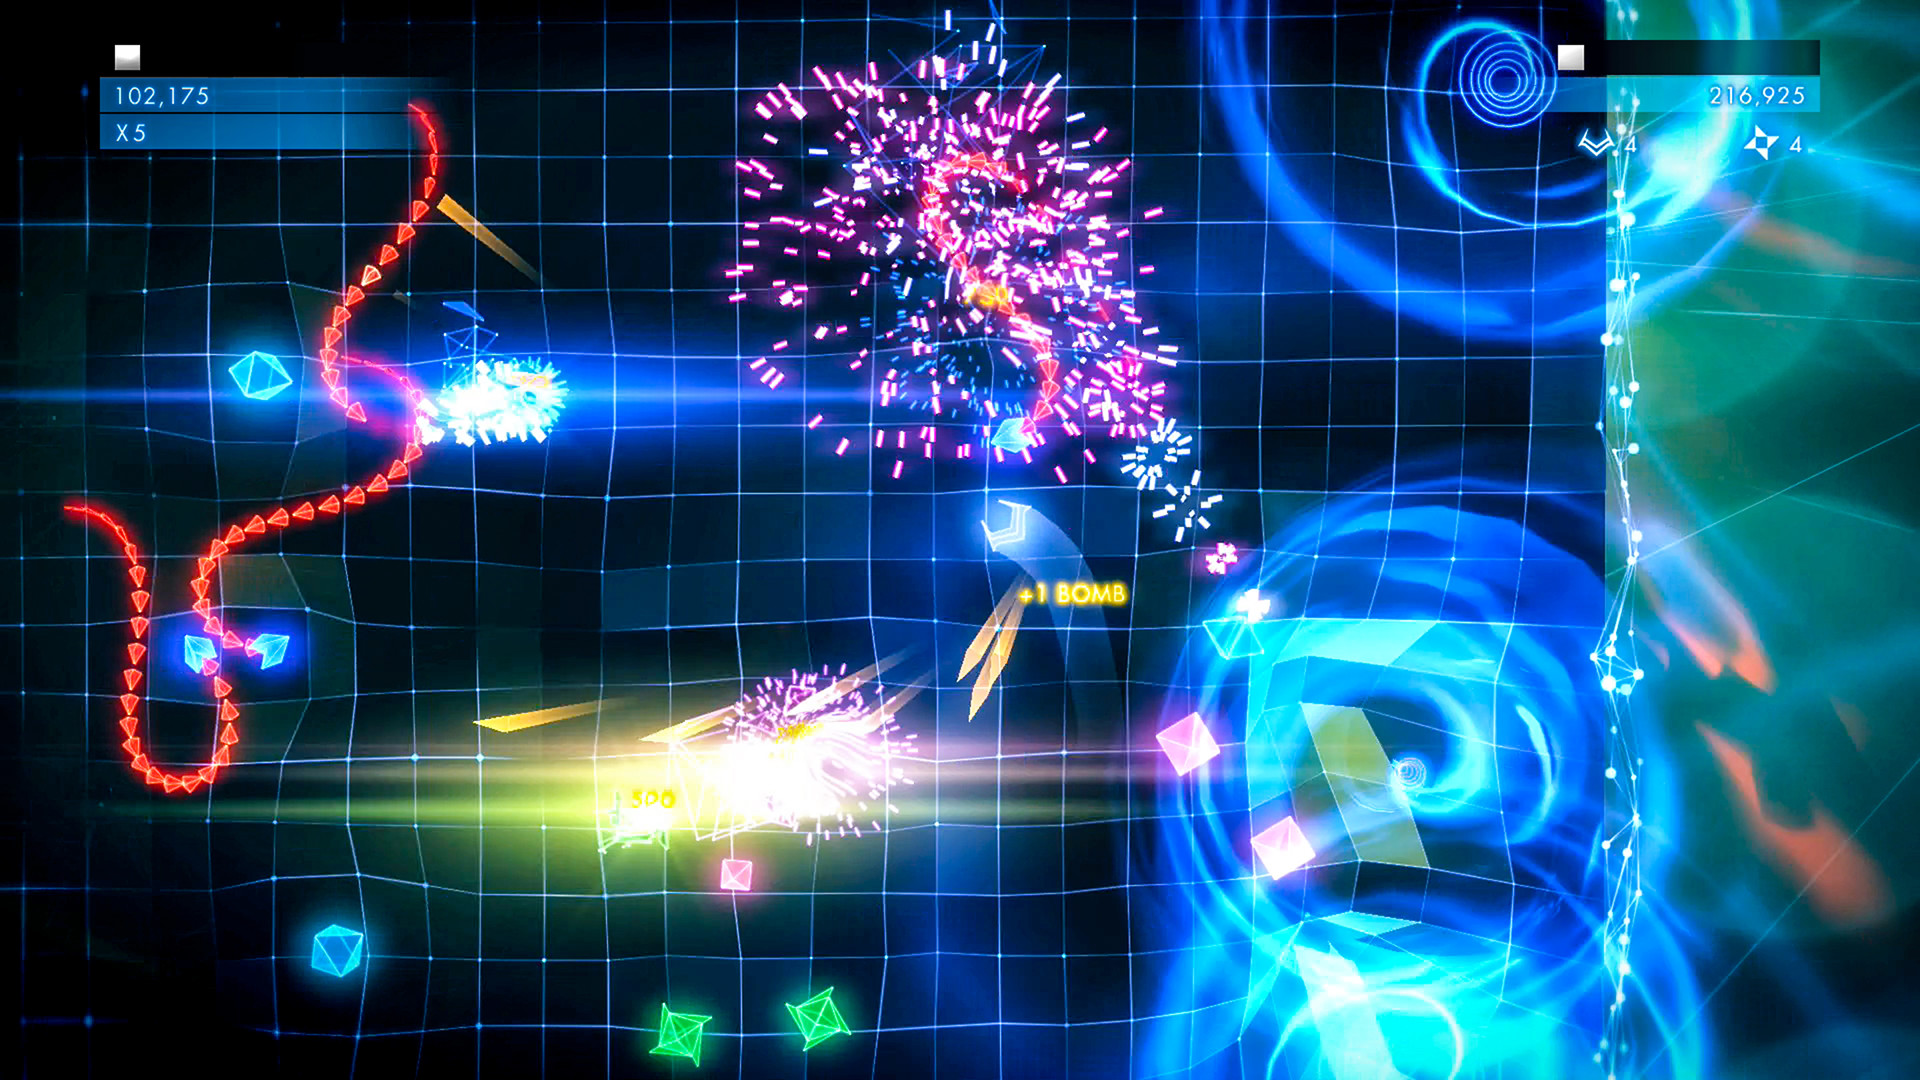
\includegraphics[width=1\columnwidth]{img/geometry_wars}
    \caption{Geometry Wars fand sich erstmals 2003 als Easter Egg in dem Spiel \textit{Project Gotham Racing} (Microsoft Game Studios). Aufgrund der großen Beliebtheit entstanden mehrere Nachfolger, zuletzt 2016 mit \textit{Geometry Wars 3: Dimensions Evolved} (Activision). (Quelle: Steam)}
    \label{fig:geometry_wars}
\end{figure}

Bei der Umsetzung orientieren wir uns in Teilen an einer in der Industrie gemeinhin akzeptierten und in der von \textit{Gregory} in~\cite[]{Gre19} beschriebenen \textit{Game Engine Architektur}, reduzieren jedoch bewusst die Anzahl der Abstraktionsschichten und verzichten auf Systeme wie Tooling, Sound oder Scripting (vgl.~\cite[\textbf{Figure 1.16}, 39]{Gre19}), so dass die \textit{Hard Architecture}~\cite[]{RM04} als technischer Unterbau einem Framework entspricht, welches Schnittstellen für benötigte Hardware und andere Subsysteme bereitstellt.
Das eigentliche Spiel wird im weiteren Verlauf von diesen Schnittstellen Gebrauch machen, für das Framework damit aber zu einer \textit{Black Box}~\cite[]{RB88}.\\

Wir stellen im Folgenden die Architektur von dem mit \textbf{helios}\footnote{
    Helios, der ``scharf vor allen mit strahlenden Augen umherblickt`` (\textit{Homers Ilias}, 14. Gesang), ist in der griechischen Mythologie der Sonnengott.
} getauften Framework vor.
Dabei berücksichtigen wir, dass es sich um einen in der Entwicklung befindlichen Prototypen handelt.
Die Software wird im Rahmen eines agilen \textit{Tracer Bullet Development}-Prozess~\cite[50 f.]{TH20} nötige Anpassungen erfahren, damit die im weiteren Verlauf aufkeimenden Anforderungen an das Gesamtsystem verhältnis- und zweckmäßig unterstützt werden können.
Wir gehen hier in Abschnitt~\ref{sec:projektdaten} noch einmal gesondert drauf ein.\\

Außerdem werden Probleme und Schwierigkeiten bei der bisherigen Umsetzung behandelt.
Diese ergeben sich durch den Umstand, dass das in vergleichsweise kurzer Zeit zu erstellende Softwareprodukt nicht nur anhand bekannter \textit{objektiver} Maße bewertet werden soll (etwa der Fehleranzahl, Software-Designentscheidungen, Kopplungsgrad der Objekte etc.), sondern auch anhand \textit{subjektiver} Maße~\cite[385]{Bal08}.\\
Zwar ist keine Klassifizierung des fertigen Produkts in Nutzungsqualitätsmerkmale angedacht\footnote{bspw. ``Nutzungsqualität nach ISO/IEC 9126``,~\cite[466]{Bal08}; Studien und Untersuchungen u.a. bei~\cite[]{AZMK17},~\cite[]{Ber10}}.
Trotzdem soll als Ergebnis nicht nur ein technisch durchdachtes, sondern auch ein für den Anwender angenehm zu bedienendes Softwareprodukt entstehen.
Diese Art User Experience werden wir im weiteren Verlauf eher unscharf, aber mit dem in diesem Bereich durchaus üblichen und allgemein akzeptierten Begriff des \textit{Game Feel}~\cite[]{Swi08} umschreiben: Einem möglichst \textit{angenehmen} und in jeglicher Hinsicht \textit{positiven Spielerlebnis}.

\begin{figure}[!h]
    \centering
    
\includegraphics[width=0.5\columnwidth]{img/helios_logo}
    \caption{Das helios Projekt-Logo.}
    \label{fig:helios_logo}
\end{figure}
